\documentclass[12pt,a4paper]{article}

\setlength{\parindent}{0.1 in}
%\setlength{\parskip}{0.1 in}
\setlength{\oddsidemargin}{0.25 in}
\setlength{\evensidemargin}{-0.25 in}
\setlength{\topmargin}{-0.5 in}
\setlength{\textwidth}{7.0 in}
\setlength{\textheight}{9.5 in}
\setlength{\headsep}{0.45 in}

%\usepackage[fleqn]{amsmath}
%\usepackage{amsfonts,graphicx}
\usepackage{amsmath,amsfonts,graphicx}
\usepackage[fleqn]{mathtools}
\usepackage{setspace}
\usepackage{hyperref}
\usepackage[nottoc]{tocbibind}
\usepackage{tocloft}
\usepackage[outermargin=2 in]{geometry}
\usepackage{scrextend}
\usepackage{tensor}
\usepackage{cancel}
\usepackage{slashed}


%Adding `Appendix' to the appendices
\usepackage[toc,page]{appendix}

%Add a bullet point to description items
\usepackage{enumitem}

%Mathematics
\usepackage{braket}
\usepackage{ulem}
\usepackage{xcolor}
\usepackage[font={small,it}]{caption}

\bibliographystyle{unsrt}

%New commands
%Maths
\newcommand{\beq}{\begin{equation}}
\newcommand{\eeq}{\end{equation}}
\newcommand{\bea}{\begin{align}}
\newcommand{\eea}{\end{align}}
\newcommand{\p}{\partial}
\newcommand{\trace}[1]{\mathrm{Tr}\left[#1 \right]}
\newcommand{\ptrace}[2]{\mathrm{Tr}_{#1} \left[ #2 \right]}
\newcommand{\bpmat}{\begin{pmatrix}}
\newcommand{\epmat}{\end{pmatrix}}
\newcommand{\vv}[1]{\vec{#1}}
\newcommand{\mat}[1]{\uuline{#1}}
\newcommand{\norm}[1]{\| #1 \|}
\newcommand{\op}[1]{\mathbb{#1}}
\newcommand{\vhat}[1]{\hat{\vv{#1}}}

%Renewed commands, in order for them to take arguments with automatically adjusted brackets 
\renewcommand{\dim}[1]{\mathrm{dim}\left( #1\right)}
\renewcommand{\det}[1]{\mathrm{det} \left( #1 \right)}
\renewcommand{\exp}[1] {\mathrm{exp} \left[ #1 \right]}


%\mathbb Letters
\newcommand{\identity}{\mathbb{I}}
\newcommand{\inreal}{\mathbb{R}}
\newcommand{\incomplex}{\mathbb{C}}

%Redefine Braket
\renewcommand{\braket}[1]{\left\langle #1 \right\rangle}

%Integration
\newcommand{\intd} {\mathrm{d}}

%Operators
\newcommand{\phihat}{\hat{\phi}}
\newcommand{\xhat}{\hat{x}}
\newcommand{\phat}{\hat{p}}
\newcommand{\Dhat}{\hat{D}}
\newcommand{\Hhat}{\hat{H}}
\newcommand{\ahat}{\hat{a}}
\newcommand{\bhat}{\hat{b}}
\newcommand{\chat}{\hat{c}}
\newcommand{\Phihat}{\hat{\Phi}}

%Channels
\newcommand{\channel}[3]{\mathcal{#1}^{#2 \rightarrow #3}}


%Caligraphy letters
\newcommand{\cl}[1]{\mathcal{#1}}
\newcommand{\Hilbert}{\mathcal{H}}
\newcommand{\calN}{\mathcal{N}}
\newcommand{\Lag}{\mathcal{L}}
\newcommand{\calD}{\mathcal{D}}


%Pauli
\newcommand{\Xhat}{\hat{X}}
\newcommand{\Yhat}{\hat{Y}}
\newcommand{\Zhat}{\hat{Z}}
\newcommand{\PauliX}{\bpmat 0 & 1 \\ 1 & 0 \epmat}
\newcommand{\PauliZ} {\bpmat 1 & 0 \\ 0 & -1\epmat}



%Gell-Mann matrices
\newcommand{\GMone} {\bpmat 0 & 1 & 0 \\ 1 & 0 & 0 \\ 0 & 0 & 0 \epmat }
\newcommand{\GMsix}{\bpmat 0 & 0 & 0 \\ 0 & 0 & 1\\ 0 & 1 & 0\epmat}

%Density matrices
\newcommand{\rhotwo}{\bpmat 1 & e^{-it} \\ e^{it} & 1 \epmat}
\newcommand{\rhothree} {\bpmat 1 & e^{it} & e^{2it} \\
e^{-it} & 1 & e^{it} \\
e^{-2it} & e^{-it} & 1 \epmat}



%Misc
\def\dbar{{\mathchar'26\mkern-12mu d}} %a $d$ with a bar through its stem


\newcommand{\eq}[1]{$#1$}

%Undertilded quantities
\newcommand{\tildeq}{\underset{^\sim}q}
\newcommand{\tildep}{\underset{^\sim}p}

%Curly letters
\newcommand{\calE}{\mathcal{E}}

\newcommand{\Nhat}{\hat{N}}

%Wave vector shortening
\newcommand{\kvec}{\vv{k}}












\begin{document}
\title{Error Correction Lecture 2 }
\author{with Dan Browne}
\maketitle
\tableofcontents

\section{Correcting Errors of the Shor Code}
Recall that the concatenated Shor code has the following initialisation circuit. 

\begin{figure}[!ht]
  \caption{Shor code initialisation diagram.}
  \centering
    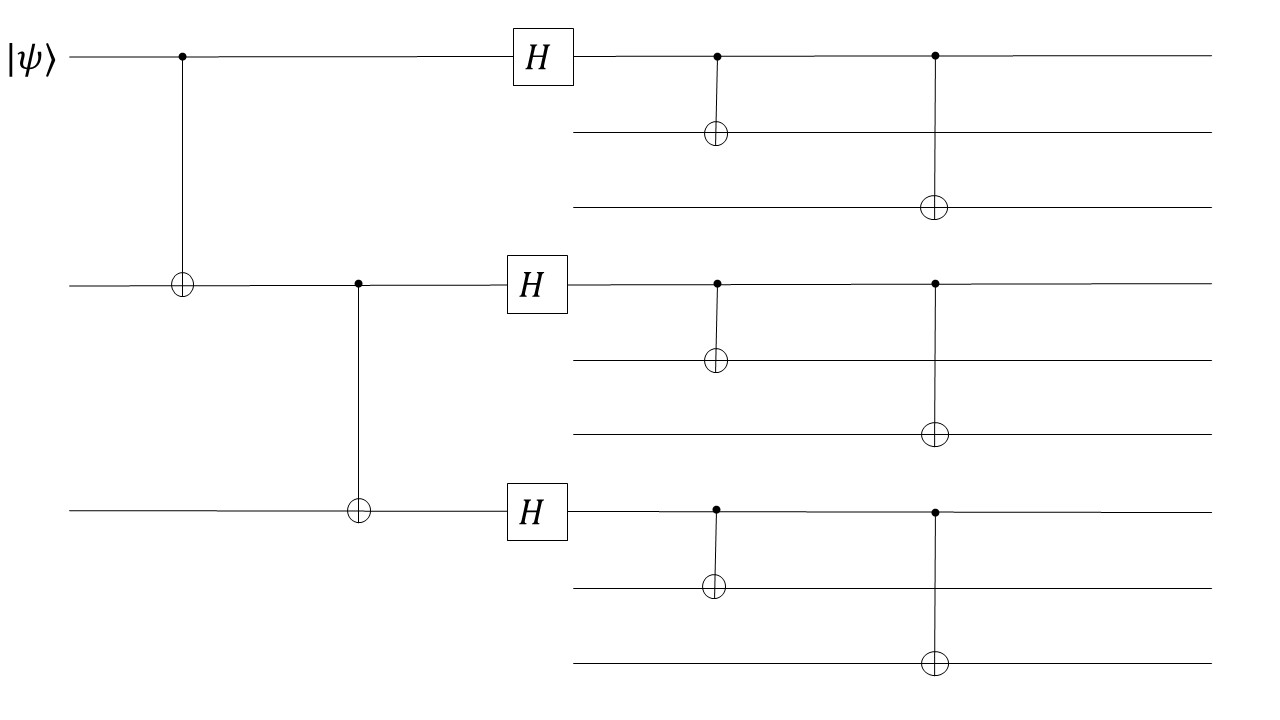
\includegraphics[width=\textwidth]{Shor_Code_Initialisation.jpg}
\end{figure}

For an error represented by the operator
\beq
X_1 = XII III III
\eeq
we get
\beq
X_1 \ket{0}_L = \left( \ket{100} + \ket{011} \right) \left( \ket{000} + \ket{111} \right)^{\otimes 2}
\eeq
\beq
X_1 \ket{1}_L = \left( \ket{100} - \ket{011} \right) \left( \ket{000} - \ket{111} \right)^{\otimes 2}
\eeq
This error is detected by the $Z_1$ and $Z_2$ parity measurements. In fact, we can write down the following table for error corrections, 
\begin{tabular}{ccc}
$Z_1Z_2$ & $Z_4Z_5$ & $Z_7Z_8$ \\
$Z_2 Z_3$ & $Z_5 Z_6 $ & $Z_8 Z_9$ \\
$(Z_3Z_1)$ & $(Z_4Z_6)$ & $(Z_7 Z_9)$
\end{tabular}
We have written the last row in brackets because just as before, it can be constructed from the other two rows and is thus superfluous. Note however that we cannot correct for two bitflip errors. The correction would introduce a factor of $-1$ on the $\ket{1}_L$ state. 

However, we know that the operator $X_1 X_2 X_3 = \bar{Z}$. This error is undetectable. As a consequence, we cannot detect any errors that happen on adjacent bits. 

In general, we want
\beq
\mbox{error} \cdot \mbox{error correction} = \identity
\eeq

\section{Phase errors}
Let us introduce the error $Z_1$. It has the following effect:
\beq
Z_1 \ket{0}_L = \left( \ket{000} - \ket{111} \right) \left( \ket{000} + \ket{111} \right)^{\otimes 2}
\eeq
\beq
Z_1 \ket{1}_L = \left( \ket{000} + \ket{111} \right) \left( \ket{000} - \ket{111} \right)^{\otimes 2}
\eeq
We can detect this error with the operator $XXXIIIIII$. It has the following effect:
\beq
XXX \left( \ket{000} \pm \ket{111} \right) = \pm \left( \ket{000} \pm \ket{111} \right)
\eeq
which enables us to see where the error has introduced a sign error. We get a negative eigenvalue for the error $XXX = \bar{Z}$. But there is a problem. Since this error is a logical operator, its detection would allow us to distinguish between $\ket{0}_L$ and $\ket{1}_L$. We can't allow this, since it would collapse any superposition. So instead, we measure $X_1 X_2 X_3 X_4 X_5 X_6$. That is, measure two out of three registers. This will check the parity between the first three and the middle three states. So we get the error detection measurements
\begin{tabular}{c}
$X_1 X_2 X_3 X_4 X_5 X_6$ \\
$X_1 X_2 X_3 X_7X_8 X_9$ \\
$(X_4 X_5 X_6 X_7 X_8 X_9)$
\end{tabular}
This can detect a single $Z$ error on every single qubit. We find the following syndrome table, using the three measurements above
\begin{tabular} {ccc}
$Z_1$ & $Z_2$ $Z_3$ \\ \hline
-- & -- & -- \\
-- & -- & -- \\
+ & + & + 
\end{tabular}
But notice that the syndrome looks the same for all three measurements! This means that we cannot distinguish between them. Say we detect $Z_2$, but we then implement the correction $Z_1$. Notice, however that the two commute. So we have
\beq
Z_2 \cdot Z_1 \ket{0}_L = \ket{0}_L
\eeq
\beq
Z_2\cdot Z_1 \ket{1}_L = \ket{1}_L
\eeq
So it works! This is the same as for the error detection operators for single bitflip errors. 

This phenomenon is called \textbf{degeneracy}. We have both non-degenerate and degenerate code. 

A non-degenerate code means that every possible correctable error has a unique syndrome. This is the case for all classical codes. 

It is, understandably, easier to prove things for non-degenerate codes. Thus, some quantum questions are still completely open systems. 

\section{Slight Generalisation}
We shall here look at the properties of Pauli operators and their tensor products. We shall use them extensively throughout the course, 
and most likely all of their properties. 

The Pauli operators are $I, X, Y, Z$. We include the identity $I$ since some of the properties include it. 

The Pauli operators have the following operators. 
\begin{itemize}
\item \textbf{All unitary} we find that for every Pauli operator, 
\beq
U^{-1} = U^\dagger = U
\eeq
\item \textbf{All Hermitian} we find
\beq
U^\dagger = U
\eeq
\item  \textbf{All are self-inverse} that is, 
\beq
U = U^{-1}
\eeq
\item \textbf{Recursive property} we can write
\beq
Y = i XZ
\eeq
Then, 
\beq
Y \ket{\psi} = i XZ \ket{\psi}
\eeq
so that a $Y$-error can be written in terms of a bitflip and phase error. The $i$ is a global phase which we can ignore. 
\item \textbf{Commute or anti-commute} All Pauli matrices anti commute. That is
\beq
\{U_i, U_j\} = 0 \mbox{ if } i \neq j
\eeq
\item \textbf{All are traceless} except for $I$. 
\item \textbf{Tensor products of Pauli matrices commute} we find that 
\beq
[X\otimes X, Z \otimes Z] = 0
\eeq

\end{itemize}
The last property means that we can always correct for a combination of errors. It means that the following statements are equivalent:
\beq 
X_E Z_E X_C Z_C
\eeq
\beq
X_E X_C Z_E Z_C
\eeq
where $E$ stands for error and $C$ stands for correction. That is, it doesn't matter in which order we detect and correct the errors since all the operators anti-commute, which just introduces a global phase. 

\section{Arbitrary errors}
Claim: We can correct for arbitrary, unitary errors. Any operator which is a tensor product of Paulis can be written $O_XO_Z$ where $O_X$ contains $X$ and $I$, and $O_Z$ contains $Z$ and $I$. 
For example, we can derive all possible $Y$ errors, 
\beq
YZIX = i(XIIX)(ZZII)
\eeq
In fact, the Pauli operators form a basis for $2^N \times 2^N$ matrices that live in $\mathbb{C}^{2^N\times 2^N}$. Any $2\times2$ matrix can be written as
\beq
O = a I + bX + cY + dZ
\eeq
To check whether they actually form a basis, we can make use the Hilbert-Schmidt inner product. 
\beq
\braket{A,B} = \trace{AB}
\eeq
which can be thought of as an orthogonality condition but for matrices. If you find a set of $D$ operators with zero Hilbert-Schmidt product where $D$ is also the dimension of the space where they live, you have a basis. 

\section{Measuring Pauli's}
We can device a circuit for measuring the Pauli operators. For a number of $n$ qubits, we can imagine a projector
\beq
P = P_1 \otimes P_2 \otimes P_3 \otimes \ldots \otimes P_n
\eeq
This circuit would simply look like projectors acting on the individual qubits. 

We know that all eigenvalues of $X,Y,Z$ are $\pm 1$. If we have
\beq
P \ket{\psi} = \ket{\psi}
\eeq
we measure a $+1$, and if we have
\beq
P\ket{\psi} = - \ket{\psi}
\eeq
we measure $-1$. 

\end{document}